\chapter{Results}
\label{chap:res}
In this section we will present and discuss the results from the experiments on the REST implementation. The experiments were conducted on an Intel(R) Xeon(R) Gold 6426Y processor with 500 GB RAM. Samples from the Porto dataset are used as data.

To describe different variants of REST, labels for each variant have been created. The spatial filter variant is denoted by the suffix \textit{-SFX}, where \textit{X} is the window size in meters. The Sakoe-Chiba band is denoted by the suffix \textit{-BNDX}, where \textit{X} is the band size. The KNN variant is denoted by the suffix \textit{-KNNX}, where \textit{X} is the number of MRTs selected. An example label can be \textit{REST-SF75-KNN3-BND20}, this represents REST using a spatial filter with window size $75\times75 m^2$, selecting the 3 best MRTs, and applying a Sakoe-Chiba band of size 20 to each Max DTW calculation.

\section{Compression Ratio and Runtime}
These experiments have been executed by first building a reference set with a sample size of 10K, to then use the reference set for compression. The trajectories in the sample used to build the reference set were excluded from the later compression, since they would have a much higher compression ratio than other trajectories.

\begin{figure}[t]
    \begin{minipage}{0.99\linewidth}
        \centering
        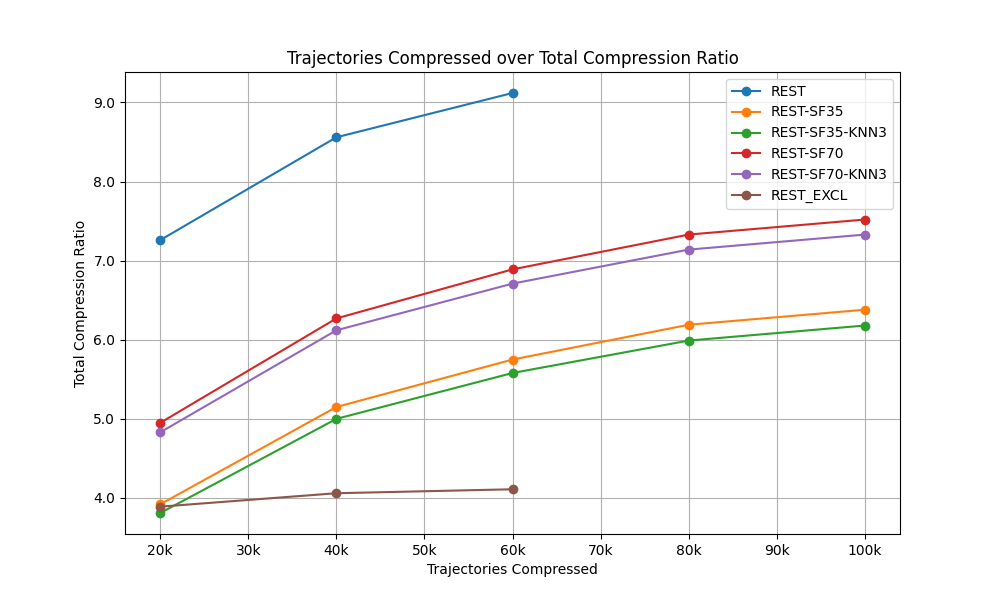
\includegraphics[height=7cm, keepaspectratio]{./figures/tot_compression.png}
        \caption{Total Compression Ratio over trajectories compressed. The reference set was constructed using a sample size of 10K.}
        \label{fig:n_compression}
    \end{minipage}
\end{figure}

In figure \ref{fig:n_compression} it is clear that REST has the best compression ratio. It has a total compression ratio of 9.12 for 60K compressed trajectories, which is high. The spatial filter variants have a lower compression ratio, but it increases with a larger window size. This is expected because REST can be seen as having an infinitely large window size. The KNN variants in combination with spatial filter shows promising results as they only slightly reduce the compression ratio compared to spatial filter with no KNN. KNN used directly on REST did not show promising results and is not shown in the results. This is likely because REST uses all reference trajectories to search for MRTs, selecting a handful early in the process seems to miss out on better suggestions.

In general the total compression grows as more trajectories are compressed. This is because the number of compressed trajectories grows larger in relation to the set size. From equation \ref{eq:tot_cr}, this represents \textit{points\_in\_set} becoming smaller compared to \textit{all\_points}. In the case where the amount of compressed trajectories keeps growing, the size of the reference set would eventually become negligible, causing the total compression to approach the average compression. The average compression ratio (not shown), stays near the same level for all variants, around 14.5 for REST. Moreover, the amount of compressions needed to make the reference set negligible is much larger than any realistic use case. The result in our experiments is that the total compression grows slower and slower.

XREST has a much slower growth than the other variants, this is because XREST has a smaller reference set. Thereby, noticing less of a change as the number of trajectories compressed increase. It also has a much lower compression ratio than REST. This indicates in combination with the exclusive strategy of XREST indicates that the reference set has low coverage. XREST needs a larger sample size in order to gain coverage, experiments covering this, are discussed in section \ref{sec:sample_size}.

\section{Sample Size testing}\label{sec:sample_size}